\section{What is a Convolutional Nerual Network}
\label{sec:cnn_theory}
This section describes what a \gls{cnn} is and what structure was used for creating the iris recognition \gls{cnn}. The section is based mainly on \cite{Karpathy2016a} and \cite{Nielsen2015}.

\subsection{Convolution}
A \gls{cnn} is type of Nerual Network that is especially good for image recognition. Instead of the input being fully connected it operates by using a kernel instead. A kernel can be seen as a small window which moves through the input image. It performs an operation known as a convolution where the coefficients, also known as weights, of the kernel are multiplied with the pixel it is covering and summing the value. A 1D example of this is shown in \autoref{fig:kernel_convolution_example} where a kernel of size 3 with weights $\begin{bmatrix} 1 & 0 & -1 \end{bmatrix}$ are convolved through bottom rows which produces the top rows. Two other concepts are also shown in the example; stride and zero padding. Stride is the amount the kernel moves each time. The left example has a stride of $1$ and the right example has a stride of $3$. Zero padding is when pixels with value $0$ are added at the edge of the image. This is done to ensure that the convolution can actually be made on all pixel because otherwise only one convolution would be possible in the example with a stride of 3. It also has the benefit of keeping the dimensions of the input image and output image the same when the stride is 1, as convolution otherwise shrinks the image. 

\begin{figure}[h]
\centering
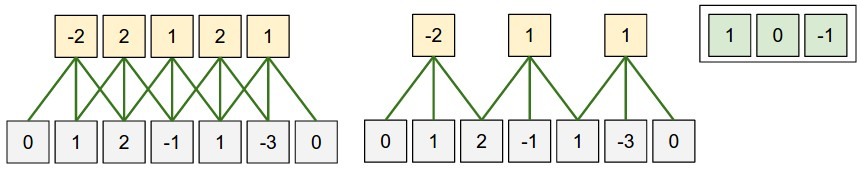
\includegraphics[width=0.90\textwidth]{kernel_convolution_example.jpeg}
\caption{Example of a kernel in a \gls{cnn} \citep{Karpathy2016a}}
\label{fig:kernel_convolution_example}
\end{figure}

The output of the convolution creates a new image. This image becomes the input of an activation function. An activation can be though of as how much should the neuron fire, e.g how active is it. A common activation function for \gls{cnn} is the \gls{relu}, \autoref{eq:ReluFunction}, that gives an output of $x$ if the $x$ is positive and 0 otherwise. This activation function has proved to be consistently better and faster for deep neural networks than the previously popular sigmoid activation function.  
\begin{eqnarray}
\label{eq:ReluFunction}
f(x) = max(0,x)
\end{eqnarray}

\subsection{Activation function/feature maps}
The output of the convolution is the hidden layer and is called a feature map. An example is shown in \autoref{fig:cnn_kernal_illustration} where a kernel of $5x5$ is used on a input image of $28x28$ to produce a feature map of $24x24$. The dimensions can be calculated by using \autoref{eq:feature_map_size}  where $W_2$ is the width of the feature map, $W_1$ is the width of the input image, $F$ is the size of the kernel and $P$ is the amount of padding.  
\begin{eqnarray}
\label{eq:feature_map_size}
W_2 = \frac{(W_1-F+2P)}{S} +1
\end{eqnarray}
The weights of the kernel is what is being learned by the network. The kernel has what is known as shared weights and biases, as its the same weights that convolve through the whole image. This is shown in \autoref{eq:shared_weights} which is how a single neuron of the feature map in example \autoref{fig:cnn_kernal_illustration} is computed. $\sigma$ is an activation function, $b$ is the shared bias,  $w$ are the weights of the kernel with $l,m$ being their position and $a$ is the input pixel at the $j,kth$.
\begin{eqnarray}
\label{eq:shared_weights}
\sigma(b+\sum\limits_{l=0}^4 \sum\limits_{m=0}^4 w_{l,m}*a_{j+l,k+m})
\end{eqnarray}
\noindent
In other words the kernel learns to detect a feature that can be found in the image, e.g. straight lines. As a single feature is not enough for recognition, multiple kernels are used to make multiple feature maps. These new feature maps become the input of another convolution layer that can learn higher level feature, e.g. combining the vertical and horizontal feature to create a kernel that detects edges. Each convolution adds a new level of abstraction.

\begin{figure}[h]
\centering
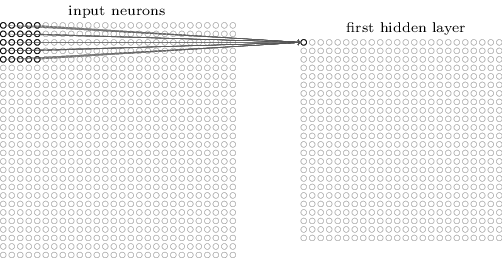
\includegraphics[width=0.90\textwidth]{cnn_kernal_illustration.png}
\caption{Example of a kernel in a \gls{cnn} \citep{Nielsen2015}}
\label{fig:cnn_kernal_illustration}
\end{figure}
\subsection{Pooling}
Pooling is an operation aften added after a convolutional layer. Like a convolution a small windows moves through the image, except it does not convolve but simply looks at the pixels in its current location and outputs a single pixel depending of the type of pooling used. Maxpooling is a common type of pooling used in \gls{cnn}s. An example of maxpooling with a windows of size $2x2$ and stride 2  is shown in \autoref{fig:maxpool_example}. This has the benefit of downscaling the spatial size of the image for faster computation and reducing overfitting.

\begin{figure}[h]
\centering
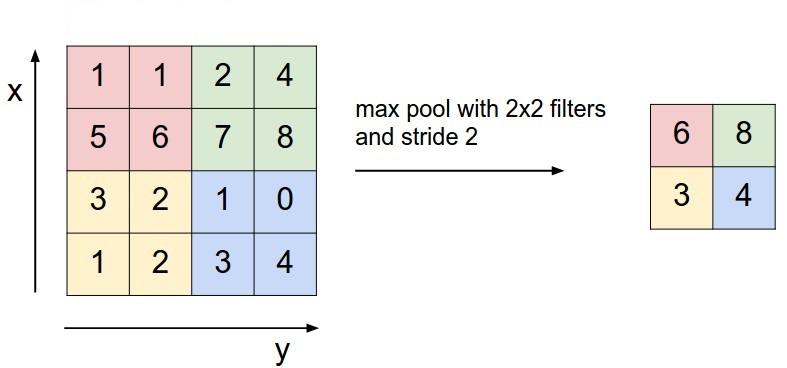
\includegraphics[width=0.90\textwidth]{maxpool_example.jpeg}
\caption{Example of maxpooling with size $2x2$ and stride 2 \citep{Karpathy2016a}}
\label{fig:maxpool_example}
\end{figure}
\subsection{Classification}
Why do we use fully connected layers for classifications


\subsection{IrisConv structure}
What and why. What is their structure? How did we implement it(python/keras)

\subsection{The structure we ended up using.}
